\documentclass[a4paper,14pt]{article}
\usepackage{float}
\usepackage{extsizes}
\usepackage{amsmath}
\usepackage{amssymb}
\everymath{\displaystyle}
\usepackage{geometry}
\usepackage{fancyhdr}
\usepackage{multicol}
\usepackage{graphicx}
\usepackage[brazil]{babel}
\usepackage[shortlabels]{enumitem}
\usepackage{cancel}
\usepackage{textcomp}
\columnsep=2cm
\hoffset=0cm
\textwidth=8cm
\setlength{\columnseprule}{.1pt}
\setlength{\columnsep}{2cm}
\renewcommand{\headrulewidth}{0pt}
\geometry{top=1in, bottom=1in, left=0.7in, right=0.5in}

\pagestyle{fancy}
\fancyhf{}
\fancyfoot[C]{\thepage}

\begin{document}
	
	\noindent\textbf{8FMA57, 8FMA58~Matemática} 
	
	\begin{center}Equação reduzida da reta - Exercícios (Versão estudante)
	\end{center}
	
	\noindent\textbf{Nome:} \underline{\hspace{10cm}}
	\noindent\textbf{Data:} \underline{\hspace{4cm}}
	
	%\section*{Questões de Matemática}
	
	
    \begin{multicols}{2}
		\begin{enumerate}
    		\item Encontre o coeficiente angular de cada uma das retas que passam pelos pontos dados e depois obtenha a sua equação reduzida.
    		\begin{enumerate}[a)]
    			\item (0; 4) e (1; 4). \\\\\\\\\\\\\\\\\\\\\\\\\\\\
    			\item (0; 3) e (5; 3). \\\\\\\\\\\\\\\\\\\\\\\\\\\\
    			\item (2; 2) e (0; 3). \\\\\\\\\\\\\\\\\\\\\\\\
    			\item (-2; 4) e (0; 6). \\\\\\\\\\\\\\\\\\\\\\\\
    		\end{enumerate}
    	    \item Faça os gráficos das retas de equação.
    	    \begin{enumerate}[a)]
    	    	\item $x = -5$ \\\\\\\\\\
    	    	\item $x = 0$ \\\\\\\\\\\\\\\\\\\\\\\\
    	    	\item $y = 7$ \\\\\\\\\\\\\\\\\\\\\\\\
    	    	\item $y = -3$ \\\\\\\\\\\\\\\\\\\\\\\\\\
    	    \end{enumerate}
            \item Faça um esboço do gráfico das retas que passam pelos pontos:
            \begin{enumerate}[a)]
            	\item (2; 3) e (3; 5). \\\\\\\\\\\\\\\\\\\\\\\\
            	\item (-3; 2) e (5; 6). \\\\\\\\\\\\\\\\\\\\\\\\
            	\item (6; 0) e (0; 9). \\\\\\\\\\\\\\\\\\\\\\
            	\item (4; -2) e (5; 7). \\\\\\\\\\\\\\\\\\\\\\\\
            \end{enumerate}
            \item Encontre as equações reduzidas de cada uma das retas desenhadas no exercício anterior.
            \begin{enumerate}[a)]
            	\item ~ \\\\\\\\\\\\\\\\\\\\\\\\
            	\item ~ \\\\\\\\\\\\\\\\\\
            	\item ~ \\\\\\\\\\\\\\\\\\\\\\\\
            	\item ~ \\\\\\\\\\\\\\\\\\\\\\\\
            \end{enumerate}
            \item Quais são os pontos da reta $r: y = x - 2$ cujas distâncias até $A = (2; 4)$ valem 4 unidades? Qual a distância de $A$ até $r$? \\\\\\\\\\\\\\\\\\
            \item Um paralelogramo $ABCD$ tem vértices $A = (0;0)$, $B = (6;0)$ e $D = (2; 3)$. Encontre a equação de reta $\stackrel{\leftarrow\rightarrow}{BC}$ \\\\\\\\\\\\\\\\\\\\\\\\
            \item Sabendo que os coeficientes angulares e lineares de uma reta são raízes da equação $x^2 - 5x - 7 = 0$, encontre a ordenada do ponto da reta cuja abscissa vale 1. \\\\\\\\\\\\\\\\\\\\\\\\\\\\\\\\\\\\
        	\item Qual o valor de $p$ para que a reta \\
        	$(3 - p)x + (3p - 1)y + 9p - 5 = 0$ \\
        	intercepte perpendicularmente o eixo $x$? Encontre o ponto de intersecção para esse caso. \\\\\\\\\\\\\\\\\\\\\\\\\\\\\\\\\\\\\\\\\\\\\\\\\\\\\\\\\\\\\\\\\\\\\\\\\\
        	\textbf{Desafio olímpico}\\
        	(OBMEP) No Brasil, usa-se a escala Celsius para medir temperaturas e, em outros países, usa-se a escala Farenheit. Para converter uma temperatura da escala Farenheit para a Celsius, subtrai-se 32 do valor da temperatura em graus Farenheit e multiplica-se o resultado por 5/9. QUal dos gráficos representa a relação entre as medidas de uma mesma temperatura em graus Farenheit (indicados por $^\circ$F) e em graus Celsius (indicados por $^\circ$C)\\
        	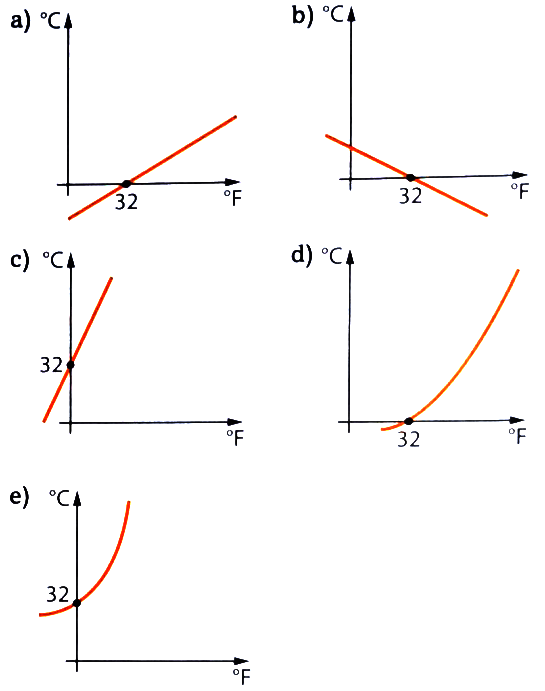
\includegraphics[width=1\linewidth]{8FMA57_imagens/imagem1}
        	\item Determine o coeficiente angular e a equação reduzida de cada uma das retas apresentadas nos gráficos a seguir:
        	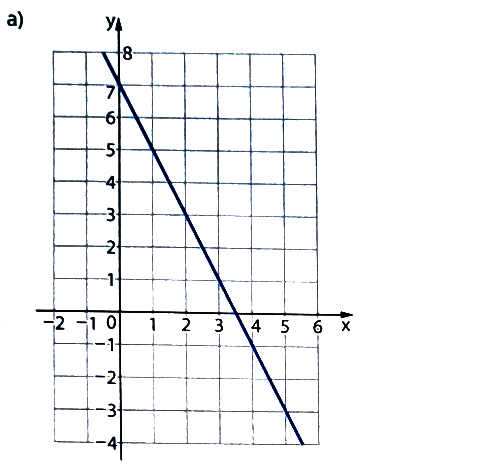
\includegraphics[width=1\linewidth]{8FMA57_imagens/imagem2}
        	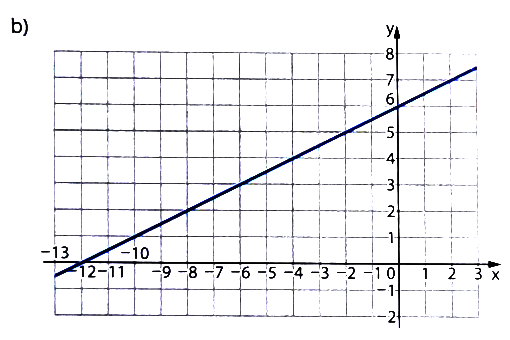
\includegraphics[width=1\linewidth]{8FMA57_imagens/imagem3}
        	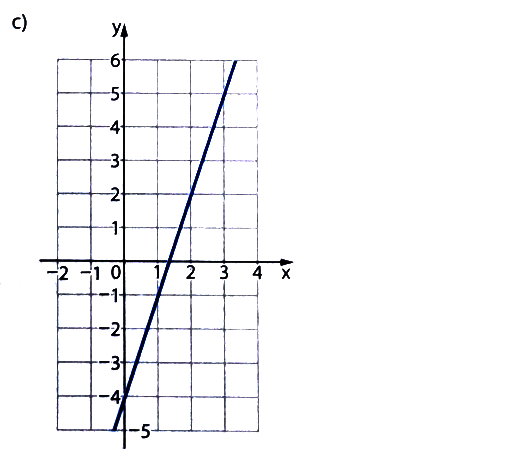
\includegraphics[width=1\linewidth]{8FMA57_imagens/imagem4}
        	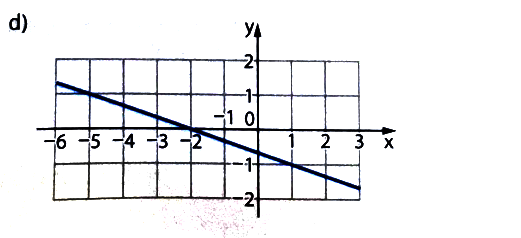
\includegraphics[width=1\linewidth]{8FMA57_imagens/imagem5} \\\\\\\\\\
        	\item Encontre a equação reduzida das seguintes retas:
        	\begin{enumerate}[a)]
        		\item $5x + 2y = 7$ \\\\\\\\\\\\\\\\\\
        		\item $2(x - 1) - 2(y + 4) = 0$ \\\\\\\\\\\\\\\\
        		\item $x^2y + x^3 + y + x = 0$ \\\\\\\\\\\\\\\\
        		\item $2x - 5y + 15 = 0$ \\\\\\\\\\\\\\\\\\
        		\item $\sqrt{3}x+\sqrt{5}y-1 = 0$ \\\\\\\\\\\\\\\\
        	\end{enumerate}
            \item Determine a equação reduzida da reta que passa pelos pontos:
        	\begin{enumerate}[a)]
        		\item (2; 3) e (-2; 6).
        		\item (0; 2) e (4; 3).
        		\item (5; -1) e (10; -3).
        		\item (2; 2) e (6; -6).
        		\item (3; -2) e (-3; -8).
        		\item (-1; 7) e (4; 2).
        	\end{enumerate}
        \end{enumerate}
    $~$ \\ $~$ \\ $~$ \\ $~$ \\ $~$ \\ $~$ \\ $~$ \\ $~$ \\ $~$ \\ $~$ \\ $~$ \\ $~$ \\ $~$ \\ $~$ \\ $~$ \\ $~$ \\ $~$ \\ $~$ \\ $~$ \\ $~$ \\
    \end{multicols}
\end{document}